\documentclass[a4paper, 14pt]{extarticle}
\usepackage[settings]{markdown}
\usepackage{minted}

% Поля
%--------------------------------------
\usepackage{geometry}
\geometry{a4paper,tmargin=2cm,bmargin=2cm,lmargin=3cm,rmargin=1cm}
%--------------------------------------


%Russian-specific packages
%--------------------------------------
\usepackage[T2A]{fontenc}
\usepackage[utf8]{inputenc} 
\usepackage[english, main=russian]{babel}
%--------------------------------------

\usepackage{textcomp}

% Красная строка
%--------------------------------------
\usepackage{indentfirst}               
%--------------------------------------             


%Graphics
%--------------------------------------
\usepackage{graphicx}
\graphicspath{ {./images/} }
\usepackage{wrapfig}
%--------------------------------------

% Полуторный интервал
%--------------------------------------
\linespread{1.3}                    
%--------------------------------------

%Выравнивание и переносы
%--------------------------------------
% Избавляемся от переполнений
\sloppy
% Запрещаем разрыв страницы после первой строки абзаца
\clubpenalty=10000
% Запрещаем разрыв страницы после последней строки абзаца
\widowpenalty=10000
%--------------------------------------

%Списки
\usepackage{enumitem}

%Подписи
\usepackage{caption} 

%Гиперссылки
\usepackage{hyperref}

\hypersetup {
	unicode=true
}

%Рисунки
%--------------------------------------
\DeclareCaptionLabelSeparator*{emdash}{~--- }
\captionsetup[figure]{labelsep=emdash,font=onehalfspacing,position=bottom}
%--------------------------------------

\usepackage{tempora}
\usepackage{amsmath}
\usepackage{color}
\usepackage{listings}
\lstset{
  belowcaptionskip=1\baselineskip,
  breaklines=true,
  frame=L,
  xleftmargin=\parindent,
  language=Python,
  showstringspaces=false,
  basicstyle=\footnotesize\ttfamily,
  keywordstyle=\bfseries\color{blue},
  commentstyle=\itshape\color{purple},
  identifierstyle=\color{black},
  stringstyle=\color{red},
}

%--------------------------------------
%			НАЧАЛО ДОКУМЕНТА
%--------------------------------------

\begin{document}

%--------------------------------------
%			ТИТУЛЬНЫЙ ЛИСТ
%--------------------------------------
\begin{titlepage}
\thispagestyle{empty}
\newpage


%Шапка титульного листа
%--------------------------------------
\vspace*{-60pt}
\hspace{-65pt}
\begin{minipage}{0.3\textwidth}
\hspace*{-20pt}\centering

\includegraphics[width=\textwidth]{emblem}
\end{minipage}
\begin{minipage}{0.67\textwidth}\small \textbf{
\vspace*{-0.7ex}
\hspace*{-6pt}\centerline{Министерство науки и высшего образования Российской Федерации}
\vspace*{-0.7ex}
\centerline{Федеральное государственное бюджетное образовательное учреждение }
\vspace*{-0.7ex}
\centerline{высшего образования}
\vspace*{-0.7ex}
\centerline{<<Московский государственный технический университет}
\vspace*{-0.7ex}
\centerline{имени Н.Э. Баумана}
\vspace*{-0.7ex}
\centerline{(национальный исследовательский университет)>>}
\vspace*{-0.7ex}
\centerline{(МГТУ им. Н.Э. Баумана)}}
\end{minipage}
%--------------------------------------

%Полосы
%--------------------------------------
\vspace{-25pt}
\hspace{-35pt}\rule{\textwidth}{2.3pt}

\vspace*{-20.3pt}
\hspace{-35pt}\rule{\textwidth}{0.4pt}
%--------------------------------------

\vspace{1.5ex}
\hspace{-35pt} \noindent \small ФАКУЛЬТЕТ\hspace{50pt} <<Информатика и системы управления>>

\vspace*{-16pt}
\hspace{47pt}\rule{0.83\textwidth}{0.4pt}

\vspace{0.5ex}
\hspace{-35pt} \noindent \small КАФЕДРА\hspace{50pt} <<Теоретическая информатика и компьютерные технологии>>

\vspace*{-16pt}
\hspace{30pt}\rule{0.866\textwidth}{0.4pt}
  
\vspace{11em}

\begin{center}
\Large {\bf Лабораторная работа № 1} \\ 
\large {\bf по курсу <<Базы данных>>}\\
\end{center}\normalsize

\vspace{8em}


\begin{flushright}
  {Студент группы ИУ9-51Б Горбунов А.\hspace*{15pt} \\
  \vspace{2ex}
  Преподаватель Вишняков И. Э.\hspace*{15pt}}
\end{flushright}

\bigskip

\vfill
 

\begin{center}
\textsl{Москва 2024}
\end{center}
\end{titlepage}
%--------------------------------------
%		КОНЕЦ ТИТУЛЬНОГО ЛИСТА
%--------------------------------------

\renewcommand{\ttdefault}{pcr}

\setlength{\tabcolsep}{3pt}
\newpage
\setcounter{page}{2}

\section{Задача}\label{Sect::task}
\par

• выбрать простейшую предметную область, соответствующую 4-5 сущностям;
    
• сформировать требования к предметной области;

• создать модель «сущность-связь» для предметной области с обоснованием выбора кардинальных чисел
связей.

\section{Практическая реализация}\label{Sect::task}
\par

\subsection{Требования к предметной области}\label{Sect::task}
В качестве предметной области был выбран сервис для поиска репетиторов.

Требования звучат так:

\begin{enumerate}
    \item Ученик может искать репетиторов по доступным предметам, сортировать их по рейтингу и количеству отзывов;
    \item Любой пользователь может создать анкету репетитора, где указывает информацию о себе: описание, рейтинг, предметы, которые он преподаёт, с ценой за час урока. Репетитор может редактировать свой профиль и отключать его показ в поиске;
    \item Ученик после занятия может оставить отзыв с оценкой. Отзывы отображаются в профиле репетитора и влияют на его средний рейтинг.
\end{enumerate}

\newpage

\subsection{Описание модели и обоснование выбора числа кардинальных связей}\label{Sect::task}
Сущности модели:
\begin{enumerate}
    \item \textbf{Students}
        \begin{itemize}
            \item \textbf{Идентификатор:} \texttt{report\_сard} (номер телефона)
            \item \textbf{Атрибуты:} \texttt{first\_name} (имя), \texttt{last\_name} (фамилия), \texttt{date\_of\_birth} (дата рождения), \texttt{encament\_date} (дата поступления), \texttt{email} (почта)
            \item Эта сущьность представляет собой собой обучающегося студента и информацию о нём.
        \end{itemize}
    
    \item \textbf{Teachers}
        \begin{itemize}
            \item \textbf{Идентификатор:} \texttt{SPIN\_code} (SPIN код преподавател)
            \item \textbf{Атрибуты:} \texttt{first\_name} (имя), \texttt{last\_name} (фамилия), \texttt{department} (кафедра), \texttt{phone\_number} (телефон), \texttt{email} (почта)
            \item Эта сущьность представляет собой собой преподавателя и информацию о нём.
        \end{itemize}

    \item \textbf{Courses}
        \begin{itemize}
            \item \textbf{Идентификатор:} \texttt{title\_of\_course}, \texttt{date\_of\_course}(название и год проведения курса)
            \item \textbf{Атрибуты:} \texttt{description} (описание предмета), \texttt{department} (кафедра), \texttt{schedule} (расписание)
            \item Эта сущьность представляет собой собой курс и его описание.
        \end{itemize}

    \item \textbf{Exams}
        \begin{itemize}
            \item \textbf{Идентификатор:} \texttt{report\_card}, \texttt{time\_stamp}, \texttt{title\_of\_course},\texttt{date\_of\_course} (табель успеваимости, дата проведения экзамена, название курса и год проведение курса)
            \item \textbf{Атрибуты:} \texttt{grade} (оценка студента), \texttt{SPIN\_code} (SPIN код преподавател)
            \item Эта сущьность представляет собой информацию о проведённом экзамене экзамене.
        \end{itemize}
\end{enumerate}

Кардинальные числа связей:
\begin{enumerate}
    \item \textbf{Students <-> Courses:}
        \begin{itemize}
            \item У одного студента может быть несколько курс, как и на курсе может обучаться несколько студентов.
            \item Связь: \textbf{«многии-ко-многим»}. Минимальная кардинальность: 0 у студента, 0 у курса (не каждый студент проходит курс, и не у каждого курса есть студент).
        \end{itemize}
    
    \item \textbf{Teachers <-> Courses:}
        \begin{itemize}
            \item Несколько преподаватель могут вести один и тот же курс, а также один преподаватель может вести несколько курсов.
            \item Связь: \textbf{«многие-ко-многим»}. Минимальная кардинальность: 0 у преподавателя, 0 у курса (у преподавателя может не быть курсов, как и не у каждого курса есть преподаватель).
        \end{itemize}

    \item \textbf{Student <-> Exams:}
        \begin{itemize}
            \item У одного студента может быть несколько экзаменов, так как он может обучаьтся на разных курсах с разными преподавателями, а каждый экзамен принадлежит только одному студенту. 
            \item Связь: \textbf{«один-ко-многим»}. Минимальная кардинальность: 0 у студента, 1 у экзамена (не у каждого студента есть экзамен, но экзамен должен быть привязан к одному студенту).
        \end{itemize}
    
    \item \textbf{Exams <-> Theachers:}
        \begin{itemize}
            \item Один экзамен может быть принят одним преподавателями, а один преподаватель может преподавать несколько экзаменов.
            \item Связь: \textbf{«один-ко-многим»}. Минимальная кардинальность: 1 у экзамена, 0 у преподавателя (для проведения экзамена нужен хотябы один преподаватель, а у преподавателя может не быть экзамена, например если он не ведёт никакой курс).
        \end{itemize}
    
    \item \textbf{Exams <-> Courses:}
        \begin{itemize}
            \item По одному курсу может быть несколько экзаменов, а у экзамена должен быть один курс.
            \item Связь: \textbf{«один-ко-многим»}. Минимальная кардинальность: 1 у экзамена, 1 у курса (у курса должен быть экзамена, как и у экзамена должен быть курс).
        \end{itemize}
\end{enumerate}

\newpage

\subsection{Модель}\label{Sect::task}
\begin{figure}[!htb]
	\centering
	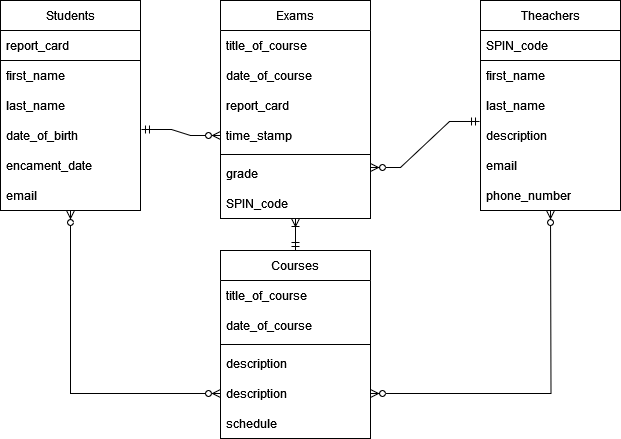
\includegraphics[width=0.8\textwidth]{schedule_lab1.png}
\caption{Модель «сущность-связь»}
\label{fig:system.png}
\end{figure}

\end{document}

